\chapter{Interference}
\label{sec:6_interference}

In this chapter, we will discuss the fundamental phenomenon of interference.
Most of you have very likely encountered interference of waves in either water, light or even sound.
We begin this chapter with a mathematical description of what happens when two waves of different frequencies interfere together.
After that, we will move to interference at the quantum level, using single photons.
Finally, we will conclude this chapter by learning that interference can occur at the level of individual qubits as well.


%%%%%%%%%%%%%%%%%%%%%%%%%%%%%%%%%%%%%%%%%%%%%%%%%%%
\section{Constructive and destructive interference}
\label{sec:6-1_constructive_and_destructive_interference}
%%%%%%%%%%%%%%%%%%%%%%%%%%%%%%%%%%%%%%%%%%%%%%%%%%%


Good starting point is to settle on the notation that will be used in this chapter.
Let's consider a wave oscillating at a single frequency, and which is propagating in time along a single dimension denoted by coordinate $x$,

\begin{equation}
    \Psi(x,t) = A \sin [\omega t-(k x+\phi_0)].
    \label{eq:simple_wave}
\end{equation}

We denote the wave with $\Psi(x,t)$.
The \textbf{\emph{amplitude}}\index{amplitude}, denoted by $A$, is the maximum value that $\Psi(x,t)$ takes.
It signifies how how much the wave is displaced from its rest state.
The symbol $\omega$ (small Greek letter ``omega'') is the \textbf{\emph{angular frequency}}\index{angular frequency}, which determines how quickly the wave oscillates.
Time is denoted by $t$.
The symbol $k$ is known as the \textbf{\emph{wave number}}\index{wave number}.
It is related to how fast the wave is propagating as well, and in three dimensions, it also gives you the direction of propagation.
Finally, $\phi_0$ (small Greek letter ``phi'') is called the initial phase of oscillations.
The angular frequency $\omega$, and the wave number $k$, are related to the period of oscillations $T$ and the wavelength $\lambda$, respectively,
\begin{equation}
    \omega=\frac{2 \pi}{T}, \qquad k=\frac{2 \pi}{\lambda},
    \label{eq:freq-period_k-wavelength}
\end{equation}

Now is a good time to have a look at some simple examples of the simple wave described by Eq.~(\ref{eq:simple_wave}).
Let's freeze the wave at time $t=0$, and for convenience we also set $\phi_0 = 0$, and only vary the wave number $k$.
The blue wave in Fig.~\ref{fig:two-waves} represents the case when $k=1$, whereas the orange one represents the case when $k=0.5$.
The wavelength is the shortest distance between two points of the where it begins to repeat itself.
We can see that decreasing the wave number $k$ by a half doubles the wavelength.
In other words, increasing the wave number ``compresses the oscillations'', while decreasing the wave number ``stretches'' them.

\begin{figure}[t]
    \centering
    \resizebox {0.6\textwidth} {!} {
    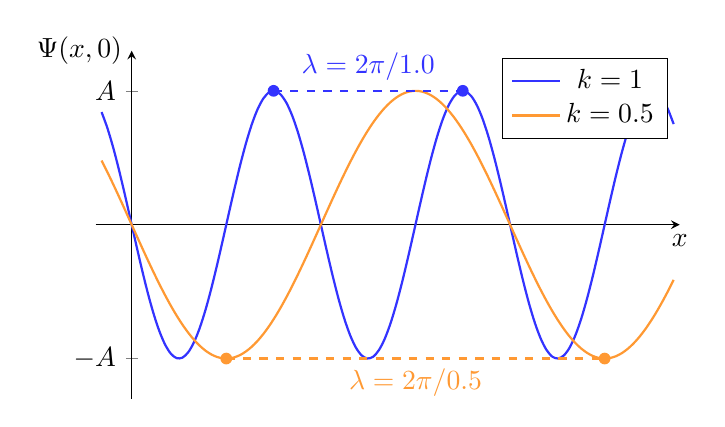
\begin{tikzpicture}
        \begin{axis}[xtick=\empty,
                    ytick={-1,1},
                    yticklabels={$-A$,$A$},
                    axis lines=middle,
                    enlarge x limits={abs=0.2},
                    enlarge y limits={abs=0.3},
                    x label style={anchor=north},
                    y label style={anchor=east},
                    xlabel={$x$},
                    ylabel={$\Psi(x,0)$},
                    width=9cm,
                    height=6cm]
        \addplot[domain=-1:18,samples=100,smooth,blue!80,thick] {sin(deg(-x))};
        \addlegendentry{$k=1$}
        \addplot[domain=-1:18,samples=100,smooth,orange!80,thick] {sin(deg(-0.5*x))};
        \addlegendentry{$k=0.5$}
        \node[circle,fill,inner sep=1.5pt,blue!80] at (axis cs:3*pi/2,1) {};
        \node[circle,fill,inner sep=1.5pt,blue!80] at (axis cs:7*pi/2,1) {};
        \draw[dashed, blue!80, thick] (axis cs:3*pi/2,1) -- node[above] {$\lambda=2\pi/1.0$} (axis cs:7*pi/2,1);
        \node[circle,fill,inner sep=1.5pt,orange!80] at (axis cs:pi,-1) {};
        \node[circle,fill,inner sep=1.5pt,orange!80] at (axis cs:5*pi,-1) {};
        \draw[dashed, orange!80, thick] (axis cs:pi,-1) -- node[below] {$\lambda=2\pi/0.5$} (axis cs:5*pi,-1);
        \end{axis}
    \end{tikzpicture}
    }
    \caption[Same frequency, different wave numbers.]{Two independent waves with $k=1$ (blue), and $k=0.5$ (orange). The time is frozen at $t=0$, and we set the initial phase to be $\phi_0=0$ for convenience.}    
    \label{fig:two-waves}
\end{figure}

Let's consider what happens when we fix the wave number but we vary the initial phase, as shown in Fig.~\ref{fig:phase-diff-waves}.
In this case, we have shifted the second wave by an initial phase of $\phi_0=\pi/2$.
Varying the initial phase has the effect of shifting the wave along the $x$ coordinate.
The wavelength of the wave remains unaffected.

\begin{figure}[t]
    \centering
    \resizebox {0.6\textwidth} {!} {
    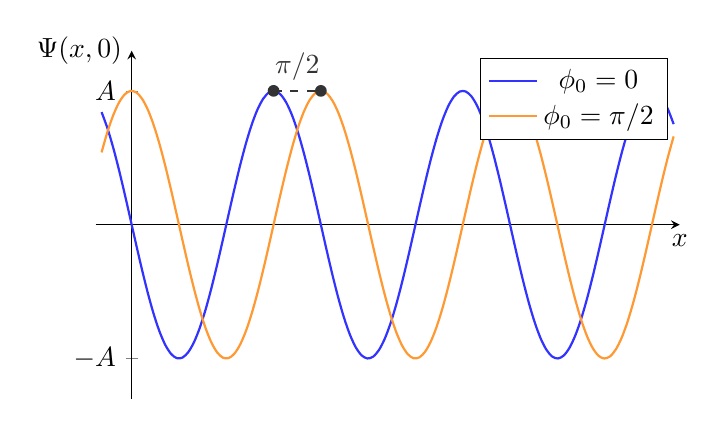
\begin{tikzpicture}
        \begin{axis}[xtick=\empty,
                    ytick={-1,1},
                    yticklabels={$-A$,$A$},
                    axis lines=middle,
                    enlarge x limits={abs=0.2},
                    enlarge y limits={abs=0.3},
                    x label style={anchor=north},
                    y label style={anchor=east},
                    xlabel={$x$},
                    ylabel={$\Psi(x,0)$},
                    width=9cm,
                    height=6cm]
        \addplot[domain=-1:18,samples=100,smooth,blue!80,thick] {sin(deg(-x))};
        \addlegendentry{$\phi_0=0$}
        \addplot[domain=-1:18,samples=100,smooth,orange!80,thick] {sin(deg(-x+pi/2))};
        \addlegendentry{$\phi_0=\pi/2$}
        \node[circle,fill,inner sep=1.5pt,black!80] at (axis cs:3*pi/2,1) {};
        \node[circle,fill,inner sep=1.5pt,black!80] at (axis cs:2*pi,1) {};
        \draw[dashed, black!80, thick] (axis cs:3*pi/2,1) -- node[above] {$\pi/2$} (axis cs:2*pi,1);
        \end{axis}
    \end{tikzpicture}
    }
    \caption[Same wavelength, different initial phase.]{Two waves with the same wavelength and frequency but different initial phases, $\phi_0 = 0$ (blue), $\phi_0=\pi/2$ (orange).}
    \label{fig:phase-diff-waves}
\end{figure}

Finally, let's add time dependence into the picture, as shown in Fig.~\ref{fig:propagating-waves}, where we have set the wave number $k=1$, and the initial phase $\phi=0$.
The angular frequency of the blue wave is set to $\omega=0.1$.
Figure~\ref{fig:propagating-waves} plots the wave at three different times $t_1$, $t_2$, $t_3$, where $t_1<t_2<t_3$.
The angular frequency of the orange wave is set to $\omega=0.2$.
We observe that the wave is propagating faster as it covers longer distance in the same amount of time.

\begin{figure}[t]
   \centering
    % \includegraphics[width=0.8\textwidth]{lesson6/w.pdf}
    \resizebox {0.6\textwidth} {!} {
    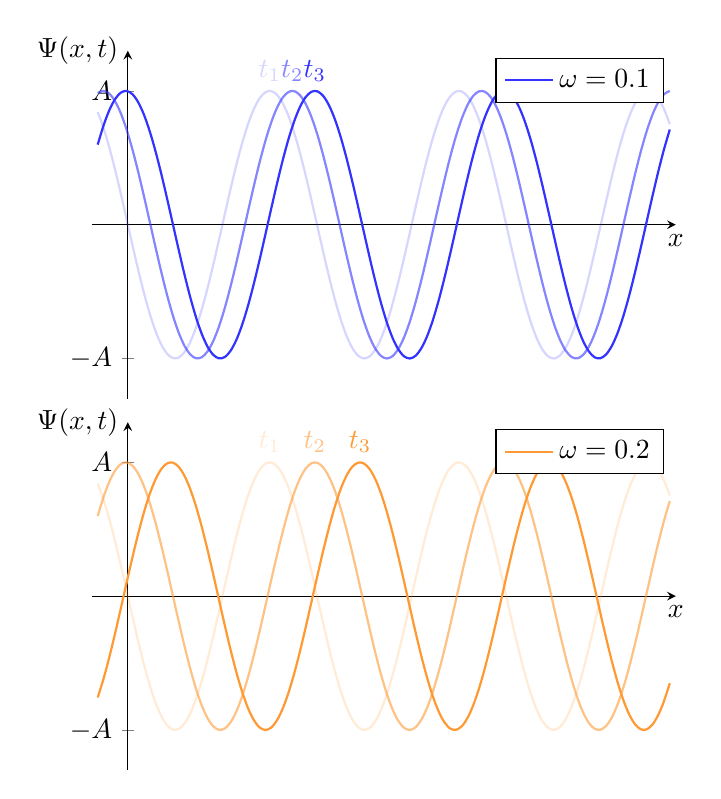
\begin{tikzpicture}
        \begin{axis}[name=plotA,
                    xtick=\empty,
                    ytick={-1,1},
                    yticklabels={$-A$,$A$},
                    axis lines=middle,
                    enlarge x limits={abs=0.2},
                    enlarge y limits={abs=0.3},
                    x label style={anchor=north},
                    y label style={anchor=east},
                    xlabel={$x$},
                    ylabel={$\Psi(x,t)$},
                    width=9cm,
                    height=6cm]
        \addplot[domain=-1:18,samples=100,smooth,blue!80,thick] {sin(deg(0.1*15-x))};
        \addplot[domain=-1:18,samples=100,smooth,blue!80,thick,opacity=0.2] {sin(deg(0.1*0-x))};
        \addplot[domain=-1:18,samples=100,smooth,blue!80,thick,opacity=0.6] {sin(deg(0.1*7.5-x))};
        \addlegendentry{$\omega=0.1$}
        \node[blue!80,opacity=0.2] at (axis cs:3*pi/2,1.15) {$t_1$};
        \node[blue!80,opacity=0.6] at (axis cs:3*pi/2+0.1*7.5,1.15) {$t_2$};
        \node[blue!80] at (axis cs:3*pi/2+0.1*15,1.15) {$t_3$};
        \end{axis}
    
        \begin{axis}[name=plotB,
                    at=(plotA.outer south west),
                    anchor=outer north west,
                    xtick=\empty,
                    ytick={-1,1},
                    yticklabels={$-A$,$A$},
                    axis lines=middle,
                    enlarge x limits={abs=0.2},
                    enlarge y limits={abs=0.3},
                    x label style={anchor=north},
                    y label style={anchor=east},
                    xlabel={$x$},
                    ylabel={$\Psi(x,t)$},
                    width=9cm,
                    height=6cm]
        \addplot[domain=-1:18,samples=100,smooth,orange!80,thick] {sin(deg(0.2*15-x))};
        \addplot[domain=-1:18,samples=100,smooth,orange!80,thick,opacity=0.2] {sin(deg(0.2*0-x))};
        \addplot[domain=-1:18,samples=100,smooth,orange!80,thick,opacity=0.6] {sin(deg(0.2*7.5-x))};
        \addlegendentry{$\omega=0.2$}
        \node[orange!80,opacity=0.2] at (axis cs:3*pi/2,1.15) {$t_1$};
        \node[orange!80,opacity=0.6] at (axis cs:3*pi/2+0.2*7.5,1.15) {$t_2$};
        \node[orange!80] at (axis cs:3*pi/2+0.2*15,1.15) {$t_3$};
        \end{axis}
    \end{tikzpicture}
    }
    \caption[Propagation of waves in time.]{Propagation of waves in time. We observe that the wave with angular frequency $\omega=0.1$ (blue) propagates more slowly compared to the wave with angular frequency $\omega=0.2$ (orange).}
    \label{fig:propagating-waves}    
\end{figure}

Having gained some intuition how the various parameters in Eq.~(\ref{eq:simple_wave}) affect the behavior of the wave, it is time to discuss what happens when two waves meet.
Let's consider a special case of two waves, $\Psi_1(x,t)$ and $\Psi_2(x,t)$, each with a different amplitude and initial phase, but both having the same frequency,
\begin{align}
    \Psi_1(x,t) & = A_1 \sin \left(\omega t+\alpha_1\right), \quad\text{where } \alpha_1=-\left(k x+\phi_1\right), \\
    \Psi_2(x,t) & = A_2 \sin \left(\omega t+\alpha_2\right), \quad\text{where } \alpha_2=-\left(k x+\phi_2\right).
    \label{eq:superposition}
\end{align}
These two waves produce a new wave given by their sum,
\begin{equation}
    \Psi(x,t) = \Psi_1(x,t) + \Psi_2(x,t).
    \label{eq:wave_superposition}
\end{equation}
This is known as the \textbf{\emph{principle of superposition}}\index{principle of superposition},
and it should look familiar.
We have in fact encountered this principle in Chapter~\ref{sec:2_quantum_states}, where we talked about superposition of two quantum state vectors.

The superposition in Eq.~(\ref{eq:wave_superposition}) will have the same form as its constituent waves,
\begin{equation}
    \Psi(x,t) = A \sin (\omega t-\alpha).
    \label{eq:resulting_wave}
\end{equation}
The question that we would like to answer is to determine how the amplitudes and initial phases of $\Psi_1(x,t)$ and $\Psi_2(x,t)$ affect the amplitude and the phase of the superpostion.
Using the trigonometric identity $\sin (a + b)=\sin a \cos b +\cos a \sin b$, we can rewrite Eq.~\ref{eq:wave_superposition} as
\begin{align}
    \Psi(x,t) & = A_1 \left( \sin\omega t \cos\alpha_1 + \cos\omega t \sin \alpha_1 \right) \nonumber\\
    & + A_2 \left( \sin\omega t \cos\alpha_2 + \cos\omega t \sin\alpha_2 \right).
\end{align}
We can group the time dependent terms together to obtain the following, 
\begin{equation}
    \Psi(x,t) = ( \underbrace{A_1 \cos\alpha_1 + A_2 \cos\alpha_2}_{\equiv A\cos\alpha} ) \sin \omega t + ( \underbrace{A_1 \sin\alpha_1 + A_2 \sin\alpha_2}_{\equiv A\sin\alpha} ) \cos \omega t.
    \label{eq:resulting_wave_2}
\end{equation}
We observe that the resulting wave $\Psi(x,t)$ does indeed oscillate with angular frequency $\omega$ as we anticipated in Eq.~(\ref{eq:resulting_wave}).
The coefficients in front of the time-dependent terms are functions of the original two waves as they depend on $A_1$, $A_2$, and $\alpha_1$, $\alpha_2$.

It would be nice to obtain a cleaner expression for the amplitude of the resulting wave $A$, and its phase $\alpha$.
We can do that by using the trigonometric identity $\cos^2\theta + \sin^2\theta=1$,
\begin{equation}
    A^2 = A^2 (\cos^2\alpha + \sin^2\alpha) = A^2\cos^2\alpha + A^2 \sin^2\alpha.
\end{equation}
We can now substitute the definition for $A\cos\alpha$ and $A\sin\alpha$ from Eq.~(\ref{eq:resulting_wave_2}), which after some rearranging yields the following expression for the square of the amplitude $A$,
\begin{equation}
    A^2 = A_1^2 + A_2^2 + 2 A_1 A_2 \cos(\alpha_2-\alpha_1).
    \label{eq:superposition-amplitude}
\end{equation}
The phase $\alpha$ can be obtained in the following way,
\begin{equation}
    \tan \alpha = \frac{A\sin\alpha}{A\cos\alpha} = \frac{A_1\sin\alpha_1 + A_2\sin\alpha_2}{A_1\cos\alpha_1 + A_2\cos\alpha_2}.
    \label{eq:superposition-alpha}
\end{equation}

We started with two initial waves that only differed in their amplitudes and initial phases.
Using the principle of superposition, we determined the mathematical description of the resulting wave $\Psi(x,t)$.
From Eq.~(\ref{eq:superposition-amplitude}), we can see that the amplitude of $\Psi(x,t)$ is determined by the amplitudes and phases of $\Psi_1(x,t)$ and $\Psi_2(x,t)$.
The last term in Eq.~(\ref{eq:superposition-amplitude}) is known as the \textbf{\emph{interference term}}\index{interference term}.
It oscillates as a function of the phase difference $\delta\equiv\alpha_2 - \alpha_1$, resulting in either positive or negative contribution to the amplitude of $\Psi(x,t)$.
When the phase difference is such that $\cos\delta>1$, the interference term contribute by increasing the amplitude $A$, which is known as \textbf{\emph{constructive interference}}\index{constructive interference}.
On the other hand, when $\cos\delta<1$, the interference term contributes negatively, situation known as \textbf{\emph{destructive interference}}\index{destructive interference}.

Let's look at the example, where the amplitudes of the initial two waves are equal, $A_1=A_2$, but their wave numbers are different.
This difference results in a phase difference, allowing us to observe both constructive and destructive interference.
The two waves have the following form,
\begin{equation}
    \Psi_1(x,t) = \sin (\omega t - k_1x), \qquad \Psi_2(x,t) = \sin (\omega t - k_2 x).
\end{equation}
The interference of these two waves is plotted in Fig.~\ref{fig:interference_example}, where we set $k_1=1.0$ (blue) and $k_2=0.8$ (orange).
The resulting wave $\Psi(x,t)$ is shown in green.
We observe that when the phase difference $\delta$ is small, which occurs in the region where $x$ is small, the two waves interfere constructively.
The amplitude of the resulting wave almost reaches all the way to $2A$.
In the region where $x$ is large however, the phase difference also increases.
We also say that the waves are ``out of phase''.
In this region, the interference is destructive.
\begin{figure}[t]
    \centering
    \resizebox {0.6\textwidth} {!} {
    \begin{tikzpicture}
        \begin{axis}[xtick=\empty,
                    ytick={-2,-1,1,2},
                    yticklabels={$-2A$,$-A$,$A$,$2A$},
                    axis lines=middle,
                    enlarge x limits={abs=0.2},
                    enlarge y limits={abs=0.8},
                    x label style={anchor=north},
                    y label style={anchor=east},
                    xlabel={$x$},
                    ylabel={$\Psi(x,t)$},
                    width=9cm,
                    height=6cm]
        \addplot[domain=-1:18,samples=100,smooth,blue!80,thick,opacity=0.5] {sin(deg(-x))};
        \addlegendentry{$k_1=1.0$}
        \addplot[domain=-1:18,samples=100,smooth,orange!80,thick,opacity=0.5] {sin(deg(-0.8*x))};
        \addlegendentry{$k_2=0.8$}
        \addplot[domain=-1:18,samples=100,smooth,newgreen,very thick] {sin(deg(-x))+sin(deg(-0.8*x))};
        \end{axis}
    \end{tikzpicture}
    }
    \caption[Superposition of two waves.]{Interference of two waves with different wave numbers.}
    \label{fig:interference_example}    
\end{figure}


%%%%%%%%%%%%%%%%%%%%%%%%%%%%%%%%%%%%
\section{Phase and group velocities}
\label{sec:6-2_phase_group_velocity}
%%%%%%%%%%%%%%%%%%%%%%%%%%%%%%%%%%%%

In this section, we will investigate the speed at which a wave propagates.
We will begin with case of waves with single frequency before moving onto more complicated scenario resulting from interference of multiple waves.

\emph{Phase velocity.}
First, let's consider a single wave of a single frequency $\omega$ propagating through space.
We saw in the previous section that we can write down such a wave as
\begin{equation}
    \Psi(x,t) = A \sin(\omega t - kx - \phi_0),
\end{equation}
where the phase at a particular point in time $t$ and space $x$ is $\theta(x,t)=\omega t-k x-\phi_0$.
The speed of propagation can be determined by inspecting any point on the wave.
This point is characterized by constant phase $\theta(x,t)$.
How fast does this point of constant phase propagate?
We need to differentiate the expression for phase with respect to time and set it equal to zero (since the phase does not change in time),
\begin{equation}
    \frac{d\theta(x,t)}{d t} = \omega - k\frac{dx}{dt} = 0.
\end{equation}
The rate of change of the position, $dx/dt$, is exactly the speed of propagation of the point of constant phase.
This quantity is called the \textbf{\emph{phase velocity}}\index{phase velocity},
\begin{equation}
    v_p \equiv \frac{dx}{dt}, \longrightarrow v_p = \frac{\omega}{k}.
    \label{eq:6-2_phase_velocity}
\end{equation}
We see that in the simple case of a single-frequency wave, the phase velocity is given as the ratio of the angular velocity $\omega$ and the wave number $k$.

\begin{figure}[t]
    \centering
    \resizebox {0.6\textwidth} {!} {
    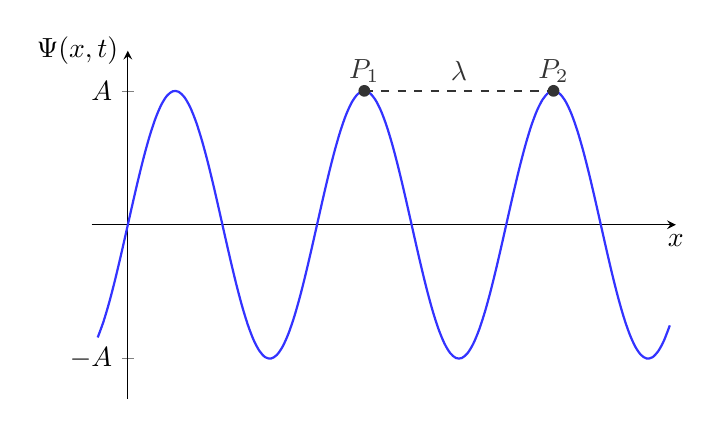
\begin{tikzpicture}
        \begin{axis}[xtick=\empty,
                    ytick={-2,-1,1,2},
                    yticklabels={$-2A$,$-A$,$A$,$2A$},
                    axis lines=middle,
                    enlarge x limits={abs=0.2},
                    enlarge y limits={abs=0.3},
                    x label style={anchor=north},
                    y label style={anchor=east},
                    xlabel={$x$},
                    ylabel={$\Psi(x,t)$},
                    width=9cm,
                    height=6cm]
        \addplot[domain=-1:18,samples=100,smooth,blue!80,thick] {sin(deg(x))};
        \node[circle,fill,inner sep=1.5pt,black!80] at (axis cs:5*pi/2,1) {};
        \node[black!80] at (axis cs:5*pi/2,1.15) {$P_1$};
        \node[circle,fill,inner sep=1.5pt,black!80] at (axis cs:9*pi/2,1) {};
        \node[black!80] at (axis cs:9*pi/2,1.15) {$P_2$};
        \draw[dashed, black!80, thick] (axis cs:5*pi/2,1) -- node[above] {$\lambda$} (axis cs:9*pi/2,1);
        \end{axis}
    \end{tikzpicture}
    }   
    \caption[Phase velocity.]{The black points represent points of same phase and are separated by the wavelength $\lambda$.}
    \label{fig:6-2_phase_velocity}
\end{figure}

We can check that the expression for phase velocity in Eq.~(\ref{eq:6-2_phase_velocity}) makes sense.
Consider one of the peaks on the wave in Fig.~\ref{fig:6-2_phase_velocity}, say point $P_1$.
This point will move to point $P_2$, covering the distance of one wavelength $\lambda$.
This represents one full oscillation of the wave, therefore the time taken to cover this distance is one period $T$.
The wave propagates at constant speed $v$, given by the ratio $\lambda/T$.
Using Eq.~(\ref{eq:freq-period_k-wavelength}), we can express this ratio in terms of the angular frequency and the wave number,
\begin{equation}
    v = \frac{\frac{2\pi}{k}}{\frac{2\pi}{\omega}} = \frac{\omega}{k} = v_p,
\end{equation}
which agrees with the phase velocity of Eq.~(\ref{eq:6-2_phase_velocity}).

\emph{Group velocity.}
How is the speed of the wave affected when the wave itself is a superposition of multiple single-frequency waves?
Let's take things slow at first by considering only two interfering waves.,
\begin{equation}
    \Psi_1(x,t) = A \sin (\omega_1 t - k_1 x), \qquad \Psi_2(x,t) = A \sin (\omega_2 t - k_2 x).
\end{equation}
We have assumed that the two waves have same amplitude, and we set the initial phase to $\phi_0=0$ for convenience.
\begin{figure}[t]
    \centering
    \resizebox {0.9\textwidth} {!} {
    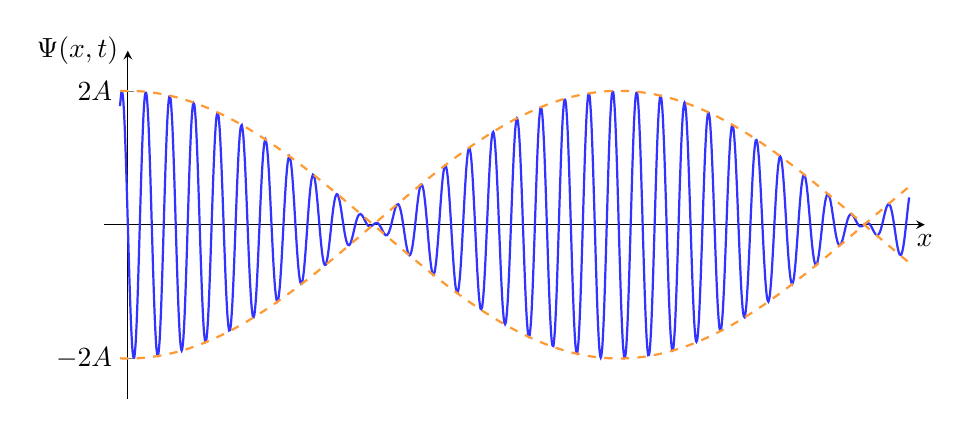
\begin{tikzpicture}
        \begin{axis}[xtick=\empty,
                    ytick={-2,2},
                    yticklabels={$-2A$,$2A$},
                    axis lines=middle,
                    enlarge x limits={abs=2},
                    enlarge y limits={abs=0.6},
                    x label style={anchor=north},
                    y label style={anchor=east},
                    xlabel={$x$},
                    ylabel={$\Psi(x,t)$},
                    width=12cm,
                    height=6cm]
        \addplot[domain=-1:100,samples=500,smooth,blue!80,thick] {sin(deg(-2*x))+sin(deg(-2.1*x))};
        \addplot[domain=-1:100,samples=500,smooth,orange!80,thick,dashed] {2*cos(deg(-0.5*(2.0-2.1)*x))};
        \addplot[domain=-1:100,samples=500,smooth,orange!80,thick,dashed] {-2*cos(deg(-0.5*(2.0-2.1)*x))};
        \end{axis}
    \end{tikzpicture}
    }   
    \caption[Group velocity.]{Superposition of two sinusoidal waves. The fast oscillations (blue solid line) are modulated by a slowly-varying envelope (orange dashed line).}
    \label{fig:6-2_superposition}
\end{figure}
Interference of these two waves results in the following superposition, 
\begin{align} 
    \Psi(x,t) & = \Psi_1(x,t) + \Psi_2(x,t) \nonumber\\
     & = A\left[\sin \left(\omega_{1} t-k_{1} x\right)+\sin \left(\omega_{2} t-k_{2} x\right)\right] \nonumber\\
    & = 2 A \underbrace{\sin \left( \frac{\omega_{1}+\omega_{2}}{2} t-\frac{k_{1}+k_{2}}{2} x \right)}_{\text{fast oscillations}} \underbrace{ \cos \left( \frac{\omega_{1}-\omega_{2}}{2} t-\frac{k_{1}-k_{2}}{2} x \right)}_{\text{slow oscillations}}.
    \label{eq:fast_slow_oscillations}
\end{align}
We see that the superposition can be split into two terms.
The first term captures the fast oscillations of the superposition at frequency $(\omega_1+\omega_2)/2$.
These fast oscillations are pictured in blue in Fig.~\ref{fig:6-2_superposition}.
Similar to the case of a single-frequency wave, we can ask the question at what speed a point of constant phase travels to obtain the \textit{\textbf{phase velocity}} for the superposition.
This information is contained in the fast-oscillation term of Eq.~(\ref{eq:fast_slow_oscillations}),
\begin{equation}
    v_p = \frac{\omega_1 + \omega_2}{k_1 + k_2}.
\end{equation}
These fast oscillations are modulated by a slowly-varying envelope as seen in by the oranged dashed line in Fig.~\ref{fig:6-2_superposition}.
This is captured by the second term in Eq.~(\ref{eq:fast_slow_oscillations}).
The frequency of these slow oscillations is $(\omega_1-\omega_2)/2$.
This term also gives rise to \textit{\textbf{group velocity}},
\begin{equation}
    v_g = \frac{\omega_1 - \omega_2}{k_1 - k_2}.
\end{equation}
The group veocity tells us how fast the entire envelope is propagating, rather than just a single point of constant phase.
The phase and group velocities of a superposition are, in general, different.
There are scenarios where one is larger than the other but also where they are equal,
\begin{equation}
    v_p > v_g, \quad v_p = v_g, \quad v_p < v_g.
\end{equation}
Real wave packets and signals are never single-frequency waves but rather results of a superposition of a number of single-frequency components.
When we talk about the speed of such a wave, we usually refer to the group velocity.
It is also the group velocity that tells us how quickly a signal carries information.

\begin{figure}[t]
    \centering
    % \includegraphics[width=0.8\textwidth]{lesson6/6-2_superpostion_many.pdf} 
    \resizebox {0.9\textwidth} {!} {
    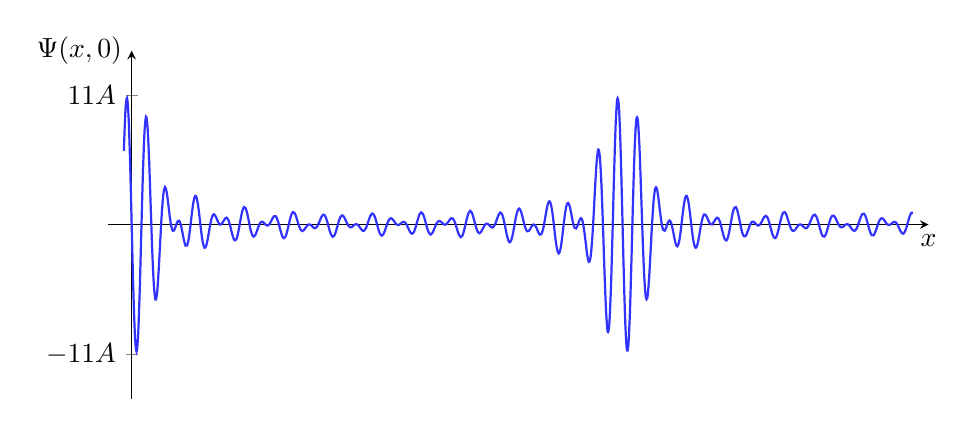
\begin{tikzpicture}
        \begin{axis}[xtick=\empty,
                    ytick={-11,11},
                    yticklabels={$-11A$,$11A$},
                    axis lines=middle,
                    enlarge x limits={abs=2},
                    enlarge y limits={abs=4},
                    x label style={anchor=north},
                    y label style={anchor=east},
                    xlabel={$x$},
                    ylabel={$\Psi(x,0)$},
                    width=12cm,
                    height=6cm]
        \addplot[domain=-1:100,samples=500,smooth,blue!80,thick] {sin(deg(-2*x))+sin(deg(-2.1*x))+sin(deg(-2.2*x))+sin(deg(-2.3*x))+sin(deg(-2.4*x))+sin(deg(-2.5*x))+sin(deg(-2.6*x))+sin(deg(-2.7*x))+sin(deg(-2.8*x))+sin(deg(-2.9*x))+sin(deg(-3.0*x))};
        \end{axis}
    \end{tikzpicture}
    }   
    \caption[Superposition of more than two waves.]{Superposition of more than two sinusoidal waves resulting in a pulse.}
    \label{fig:6-2_pulse}
\end{figure}
To complete our discussion, let's look at the case when we have more than two single-frequency components interfering together.
Let's say we have a superposition of the following form,
\begin{equation}
    \Psi(x,t) = A [\sin(-2.0x) + \sin(-2.1x) + \ldots + \sin(-3.0x)].
    \label{eq:6-2_pulse}
\end{equation}
We have assumed that we are looking at the superposition frozen in time at $t=0$, hence the simple form.
The resultant superposition is pictured in Fig.~\ref{fig:6-2_pulse}.
Unlike before, we can observe long regions where destructive interference results in almost no disturbance.
Then the constructive interference kicks in and we observe a short \textbf{\emph{pulse}}\index{pulse}.
It is these pulses that can be used to carry information at the group velocity of the superposition.


%%%%%%%%%%%%%%%%%%%%%%%%%%%%%%%%%%%%%%%%%%%
\section{Interference with single photons}
\label{sec:6-4_interference_single_photons}
%%%%%%%%%%%%%%%%%%%%%%%%%%%%%%%%%%%%%%%%%%%

% double_slit standard
\begin{figure}[H]
   \centering
    \includegraphics[width=0.8\textwidth]{lesson6/standard_double_slit.pdf}    
        \caption{The canonical two-slit experiment.}
    \label{fig:two-slit}
   
\end{figure}

I'm sure you have already seen the scenario of a double slit experiment with laser light in another of your physics classes, but let's review it again.

In this experiment we have a source of coherent light, canonically a laser. In Fig.~\ref{fig:two-slit}, the laser light is incident on a screen, where there are only two small slits where the light can go through, and then it propagates towards another screen where we detect a pattern. The pattern that we see looks something like this: we have fringes of bright light (pink in the figure), and then fringes where there is no light (blank, or white, in the figure). Why is that?  The pink lines represent the peaks of the electromagnetic waves. They are straight before coming to the screen, perpendicular to the direction of travel. After passing through the slits, they radiate out in a circular pattern.  Following the light blue lines, you can see that where the peaks from the two slits meet, the lines cross.  Those blue lines are where we get constructive interference, giving us the strong pink illumination on the screen. Halfway in between those blue lines, you can see that the wave from one slit is at its peak when the other is at its trough.  This will give us destructive interference.

% As you can see, as the light is propagating through here (follow pointer), these lines, they represent the peaks of the electromagnetic wave, whereas the space in between them represent the valleys, the troughs. So as the two waves go through these slits, they have a chance to interfere constructively or destructively. Where their peaks meet, the wave- the interference of the two waves reinforces their amplitude. On the other hand, if a peak meets a trough or a valley, then the amplitudes cancel, and here we can see these light blue lines, these are the lines along which we see constructive interference.

For example, consider the point right in the middle of the screen, as shown in Fig.~\ref{fig:two-slit-constructive}. The light coming from the top slit and light coming from the bottom slit travel the same distance. The path length of these two paths are equal, therefore there is no phase difference between the two waves coming from the top slit and the bottom slit, and we observe constructive interference. On the other hand, for the fringe above the middle, the path length for the top path is a little bit shorter than the bottom one. But the phase difference introduced for this case is exactly $2\pi$, which again, corresponds to constructive interference as we have seen in the previous section. Similarly for the top fringe in our figure, we have a phase difference of $4\pi$.
% constructive interference
\begin{figure}[H]
   \centering
    \includegraphics[width=0.8\textwidth]{lesson6/double_slit_constructive.pdf}    
        \caption{Constructive interference.}
    \label{fig:two-slit-constructive}    
\end{figure}

On the other hand, consider the paths shown in Fig.~\ref{fig:two-slit-destructive}. Along these paths, peaks meet the troughs, where the path differences are odd integer multiples of $\pi$. So for this first dark (blank white) region on the screen, we have the phase difference being $\pi$; for the second dark region on the screen, we have the phase difference being $3\pi$, and so on.

% destructive inteference
\begin{figure}[H]
   \centering
    \includegraphics[width=0.8\textwidth]{lesson6/double_slit_destructive.pdf}
        \caption{Destructive interference.}
    \label{fig:two-slit-destructive}    
\end{figure}

Now, let's consider the scenario where we attenuate the laser light to such low levels that it's only firing single photons at a time, and furthermore, the level of attenuation is so high that we can be pretty sure that there's only one photon at a time between this screen where we place the double slits, and the screen where we are recording the pattern. So, what happens? Well, we know that the photons must go through one of these slits. So, let's try covering one of them. What do we expect? If we cover the bottom one, then definitely the photons have to go through the top slit in order to hit the screen, so we expect most of the photons hitting the screen will appear in the region that's the closest to the top slit, as in Fig.~\ref{fig:two-slit-lower-blocked}. On the other hand, if we block the top slit, as in Fig.~\ref{fig:two-slit-upper-blocked}, and the photons are allowed to pass through this bottom slit, then we expect most of the photons to be recorded on the lower portion of the screen. What happens if we open both of the slits, as in Fig.~\ref{fig:two-slit-single-photon-wrong}? They can go through the top, and they can go through the bottom, so we expect something like this: we expect that the two previous distributions are just added together. Is this really what we see? Well, let's find out. 

% attenuated laser
\begin{figure}[H]
   \centering
    \includegraphics[width=0.8\textwidth]{lesson6/attenuate_laser.pdf}    
        \caption{Attenuated laser light.}
    \label{fig:two-slit-attenuated}
\end{figure}

% block bottom
\begin{figure}[H]
   \centering
    \includegraphics[width=0.8\textwidth]{lesson6/block_bottom.pdf}
    
        \caption{Pattern observed when the lower slit is blocked.}
    \label{fig:two-slit-lower-blocked}
    
\end{figure}

% block top
\begin{figure}[H]
   \centering
    \includegraphics[width=0.8\textwidth]{lesson6/block_top.pdf}
    
        \caption{Pattern observed when the upper slit is blocked.}
    \label{fig:two-slit-upper-blocked}
    
\end{figure}


% block netiher expectation
\begin{figure}[H]
   \centering
    \includegraphics[width=0.8\textwidth]{lesson6/block_neither.pdf}
    
        \caption{When single photons are used and both slits are open, is this the pattern we observe?}
    \label{fig:two-slit-single-photon-wrong}
    
\end{figure}

In fact, we see the following: we start firing photons at the screen. Originally, there's not much pattern that we can discern, as on the left side of Fig.~\ref{fig:two-slit-single-photon-pattern}, but as time progresses, more and more photons hit the screen and we can clearly see these fringes being formed, as on the right side of the figure. These fringes are the same fringes we could see before with strong laser light. Let's pause and appreciate really what's going on. We saw these fringes on the right with a strong laser light, and it wasn't very surprising. Here, somehow each individual photon knows that they still need to follow the same pattern. Still they are drawn toward the bright fringes on the screen, and they avoid the dark fringes in between. This is because of interference of different possible paths. Even though we only have a single photon between the laser and the screen, still it obeys the same rules of interference as if we had a strong laser pulse.


% block neither reality
\begin{figure}[H]
   \centering
    \includegraphics[width=0.8\textwidth]{lesson6/block_neither_reality.png}    
        \caption{In fact, when both slits are open, even single photons will create the same pattern after a large number of individual photons have accumulated.}
        \label{fig:two-slit-single-photon-pattern}

\end{figure}


\section{Interference with qubits}




We have seen how light interferes, how waves interfere, and even how single photons interfere. We can, in fact, see interference also with single qubits. Let's see how.

Consider that we have a Hadamard gate, and we apply it on the state of a qubit. We will consider two states: one is our state $\ket{0}$ which is given by the state vector (one zero), and the other is the state $\ket{1}$, which is given by its orthogonal friend (zero one), and the Hadamard gate $H$ is given by the transformation matrix,
\begin{equation}
\begin{aligned}
|0\rangle &=\left(\begin{array}{l}
1 \\
0
\end{array}\right) \quad|1\rangle=\left(\begin{array}{l}
0 \\
1
\end{array}\right) \quad H=\frac{1}{\sqrt{2}}\left(\begin{array}{cc}
1 & 1 \\
1 & -1
\end{array}\right)
\end{aligned}
\end{equation}

If we start in the state $\ket{0}$ and apply the Hadamard gate to it, we have seen that we create an equal superposition of state $\ket{0}$ and $\ket{1}$,
\begin{equation}
\begin{aligned}
|0\rangle & \longrightarrow H|0\rangle=\frac{1}{\sqrt{2}}(|0\rangle+|1\rangle)
\end{aligned}
\end{equation}
Now we can do the same thing again, we can apply another Hadamard gate to this superposition,
\begin{equation}
\begin{aligned}
H\left[\frac{1}{\sqrt{2}}(|0\rangle+|1\rangle)\right] &=\frac{1}{2}(|0\rangle+|1\rangle+|0\rangle-|1\rangle) \\
&=|0\rangle
\end{aligned}
\end{equation}
This can be seen by breaking the equation into its separate terms. From the first term, applying the Hadamard to the state $\ket{0}$ creates another superposition $\ket{0}+\ket{1}$. Applying Hadamard gate to the second term, the state $\ket{1}$ creates a superposition $\ket{0}-\ket{1}$. So after applications of two Hadamard gates, this is our state: the two $\ket{0}$ terms have the same sign and add up, or constructively interfere. The two $\ket{1}$ terms have opposite signs and cancel, or destructively interfere.
%You can see that these terms (0+1, 0-1), they both have a positive probability amplitude, plus a half, plus a half. Whereas the other two terms have opposite amplitudes, they've got plus a half, and negative a half. So the effect of that is that the probability amplitudes for ones cancel, whereas the probability amplitudes for the zeros, they constructively interfere, and we end up in a state zero which was our initial state, and this works also for state one if we use that as an initial state, but this time the cancellation of probability amplitudes happens for the zero terms, because they have plus one half minus one half, and the one terms, they constructively interfere because both of them have plus a half, plus a half probability amplitudes. So 
This may not surprise you too much. After all, applying Hadamard twice actually applies the identity, because the Hadamard gate is its own inverse.

So let's consider two different transformations. Let's call them BS1 and BS2,
\begin{equation}
B S 1=\frac{1}{\sqrt{2}}\left(\begin{array}{cc}
1 & 1 \\
1 & -1
\end{array}\right) \quad B S 2=\frac{1}{\sqrt{2}}\left(\begin{array}{cc}
-1 & 1 \\
1 & 1
\end{array}\right) \quad B S 2 \cdot B S 1 \neq I.
\end{equation}
You can see that BS1 is actually our previous Hadamard gate but let's just keep calling it BS1 for reasons that will become apparent a little bit later.  BS2 looks a little bit  like a Hadamard gate, but this time the minus is not located in the bottom right, but instead is in the top left. You can check for yourself that applying these gates in sequence is not the same thing as doing nothing. In particular, BS2 times BS1 is not equal to the identity.

But let's see what happens when we do apply them. Let's say our initial state is $\ket{1}$. We first apply the transformation BS1, then BS2, and what we get is the following
\begin{equation}
\begin{aligned}
B S 2 \cdot B S 1|1\rangle &=B S 2 \cdot \frac{1}{\sqrt{2}}\left(\begin{array}{cc}
1 & 1 \\
1 & -1
\end{array}\right)\left(\begin{array}{l}
0 \\
1
\end{array}\right) \\
&=B S 2 \cdot \frac{1}{\sqrt{2}}\left(\begin{array}{c}
1 \\
-1
\end{array}\right) \\
&=\frac{1}{2}\left(\begin{array}{cc}
-1 & 1 \\
1 & 1
\end{array}\right)\left(\begin{array}{c}
1 \\
-1
\end{array}\right) \\
&=\frac{1}{2}\left(\begin{array}{c}
-2 \\
0
\end{array}\right)=-|0\rangle=|0\rangle
\end{aligned}
\end{equation}
We apply the Hadamard gate to the vector (zero one), and after simple multiplication we get the superposition $\ket{0}-\ket{1}$. Then, we apply BS2, and what we get is in fact another translation. The probability amplitudes corresponding to state $\ket{0}$, they constructively interfere, whereas the probability amplitudes contributing towards state $\ket{1}$, they destructively interfere. Therefore the probability amplitude for state $\ket{1}$ becomes zero. The minus term that appears on the front is not important, it has no consequence because it's just a global phase, so we can just ignore it.
 
Now, let's consider an optical instrument called a \emph{Mach-Zehnder Interferometer}\index{Mach-Zehnder interferometer}\index{interferometer}, as shown in Fig.~\ref{fig:mach-zehnder}.
% Mach-Zehnder set-up
\begin{figure}[H]
   \centering
    \includegraphics[width=0.8\textwidth]{lesson6/mach_zehnder.pdf}
    
        \caption{Mach-Zehnder interferometer.}
    \label{fig:mach-zehnder}
    
\end{figure}
It consists of two beam splitters which are BS1 and BS2, two mirrors, and two detectors.  The game that we like to play with this Mach-Zehnder Interferometer is this: we feed in some light into the first beam splitter, and then we ask the questions, "When will D0 click?  When will detector D1 click? What's the intensity measured at detector D0? What's the intensity measured at detected D1?" and so on. In this particular case, we assume that we only have light coming in from the bottom, and the mirrors and beam splitters are set in such a way that the path lengths are the same. The light can be reflected from the first beam splitter, bounce off the mirror, and enter the second beam splitter, or it can be transmitted through the first beam splitter, bounce off the top mirror, hit the second beam splitter interfere with the beam coming from the bottom branch, and it will be detected either at D0 and D1. If the path lengths are the same, then for this scenario, it will always be detected in the top detector D0.

That's what happens with strong, classical light. Now, let's consider what happens when only a single photon enters our Mach-Zehnder Interferometer, as in Fig.~\ref{fig:mach-zehnder-single-photon}. Again, the single photon can be reflected at the first one or transmitted. It bounces off the mirrors, which don't really do anything except alter the path of the photon.  The two paths then recombine at the second beam splitter, and we ask the question: is the photon detected at D0 or is it detected at D1?
% Single photon Mach-Zehnder case
\begin{figure}[H]
   \centering
    \includegraphics[width=0.8\textwidth]{lesson6/mach_zehnder_single_photon.pdf}
    
        \caption{Mach-Zehnder interferometer with a single photon.}
    \label{fig:mach-zehnder-single-photon}    
\end{figure}

In addition, the Mach-Zehnder Interferometer implements our qubit. How? Where is the qubit? Well, if the photon is found in the top half of the interferometer, we say that it's in the state $\ket{0}$, as in Fig.~\ref{fig:m-z-upper}. On the other hand if it's found in the bottom half, we say that it's in the state one, Fig.~\ref{fig:m-z-lower}. 
%So here the different paths encode different computational states of the qubit.

% 0 ket top
\begin{figure}[H]
   \centering
    \includegraphics[width=0.8\textwidth]{lesson6/0_ket_botttom.pdf}
    
        \caption{$\ket{0}$ state is represented by a photon in the upper path.}
    \label{fig:m-z-upper}
    
\end{figure}

% 1 ket bottom
\begin{figure}[H]
   \centering
    \includegraphics[width=0.8\textwidth]{lesson6/1_ket_bottom.pdf}
    
        \caption{$\ket{1}$ state is represented by a photon in the lower path.}
    \label{fig:m-z-lower}
    
\end{figure}

Let's consider our initial state to be $\ket{1}$, meaning it enters our Mach-Zehnder Interferometer from the bottom half.

Now you see why we have called those previous transformations BS1 and BS2. They correspond to the mathematical description of how these beam splitters affect the probability amplitudes of our qubit~\footnote{In fact, the quantum mechanical description of a beam splitter always has to involve writing down the state of both of the input ports to the beam splitter; here, we are being a little loose with the description. BS2 in this figure shows the correct accounting for photons coming from above and below the beam splitter, but for BS1 we have ignored the fact that we need to count the number of photons coming in from both above and below it, as well.  In future courses in this sequence, you will see a more rigorous treatment.}. We proved before that if we first act on our qubit with beam splitter one, and subsequently with beam splitter two, then we know that if the initial state is in the bottom half, then the output state will always be found in the top half, meaning D0 detector always clicks, as in Fig.~\ref{fig:m-z-d0}. The situation is very similar to the previous section. Here, there is only a single photon found in the Mach-Zehnder Interferometer. A photon is a single unit. There's always just one and it can't be divided, yet somehow it knows that it has to interfere with itself and always goes towards detector D0.

Now, let's do a simple test to better understand the behavior. Let's actually put some absorbing material and block the possibility of the photon going through the lower half of the Mach-Zehnder Interferometer, as in Fig.~\ref{fig:m-z-blocked}. What do we see? Well, the photon coming from below can get reflected at BS1. If it does get reflected, then it hits the block, gets absorbed and we don't get any clicks. However, if it gets transmitted at BS1, it bounces off the upper mirror and it is incident onto the second beam splitter, where again, it has an equal probability of being reflected or passing through the beam splitter. Therefore, it has a probability of being detected by both detector D0 and the detector D1. Effectively, by blocking this path of photon in the bottom of the Mach-Zehnder Interferometer, we have prevented interference from taking place at BS2. That is why we see both possibilities D0 and D1.

\if0
\begin{equation}
B S 2 \cdot B S 1|1\rangle=|0\rangle
\end{equation}
\fi

% D0 always clicks
\begin{figure}[H]
   \centering
    \includegraphics[width=0.8\textwidth]{lesson6/d0_always_clicks.pdf}
    
        \caption{$D0$ clicks with 100\% probability.}
    \label{fig:m-z-d0}
    
\end{figure}

% block bottom path
\begin{figure}[H]
   \centering
    \includegraphics[width=0.8\textwidth]{lesson6/bottom_blocked.png}
    
        \caption[Lower path blocked.]{Lower path blocked. Because there is no photon coming from the lower path at BS2, no interference occurs, and any photon coming from above has a 50/50 chance of being directed to either detector.}
    \label{fig:m-z-blocked}
    
\end{figure}


\newpage
\begin{exercises}

\exer{Write some code to reproduce the static plot in Fig.~\ref{fig:decaying-superposition}.  Try to make your code represent the equations as nearly exactly as possible.  The plots and animations in our course were created using the Python package {\tt manim}, but your instructor may have different instructions for you.}

\exer{Write some code to reproduce the animated plot in Fig.~\ref{fig:propagating-waves}.  Try to make your code represent the equations as nearly exactly as possible.  The plots and animations in our course were created using the Python package {\tt manim}, but your instructor may have different instructions for you.}

\end{exercises}

